% !TEX root = ./main.tex
\section{GraphCoQL}\label{sec:form}

In this section we describe our formalization of GraphQL in Coq. We start by defining a schema and its properties, then the graph data model and finally we review queries and their semantics. The definitions are as close as possible with respect to the \spec{}. This eyeball correspondence between the english-written definitions and the code gives a first level of trust that our formalization is correct, following the examples of X, Y and Z. Whenever there is a mismatch we point it out and explain the reasoning behind each decision.


\subsection{GraphQL Schema}\label{subsec:schema}

First, we implement the schemas as described in the \spec{}.  A schema is ``\textit{defined in terms of the types and directives it supports as well as the root operation types for each kind of operation}''\footnote{https://graphql.github.io/graphql-spec/June2018/\#sec-Schema}. 
We represent it with a record, containing both the list of type definitions and root operation types.  The only possible root operation is querying; mutations and subscriptions are not currently implemented. \td{Not sure how to introduce the things that are not implemented: Input Object types, Descriptions (Introspection), directives, type extensions, non-null, etc. Probably just push to discussion?}

\begin{minted}{coq}
Record graphQLSchema := GraphQLSchema {
    query_type : Name;
    type_definitions : seq TypeDefinition
}.
\end{minted}

Next, type definitions are also implemented following the \spec{}. Figure \ref{fig:types_def} shows the grammar and the implementation in Coq, which tries to mimic the grammar as close as possible, in order to get a degree of trust given by an eyeball correspondence. We choose not to embed non-emptiness of fields, union members and enum members, and push the validation to a separate predicate. The reasons are that the \spec{} also repeats this validation, even when the grammar embeds this notion, and secondly, we find it simpler to reuse the existent machinery for lists.

% As can be seen from the figure, our implementation looses information about non-emptiness of fields, union and enum members. We push this validation to a posterior predicate, as well as the discussion about the reasons behind this decision, to the following paragraphs.

% As can be seen in the figure, we tried to match the \spec{}'s definition as much as possible. This eyeball correspondence gives us a degree of confidence about the implementation.  % We currently do not include the \textit{Input Object} types, as well as anything related to \textit{introspection}.

Although the previous definitions are straightforward, both the \spec{}'s grammar and the Coq implementation allow building invalid schemas. For instance, it is possible to build an object that implements scalar types or use a nonexistent type as the query type. To this end, the \spec{} includes validation rules scattered throughout the document\footnote{Most can be found in the \textbf{Type Validation} subsection of each type described in https://graphql.github.io/graphql-spec/draft/\#sec-Type-System.}.  We summarize these rules and refer to it as the \textit{well-formedness} property of a GraphQL schema.


\begin{definition}
A GraphQL schema is \textit{well-formed} if it satisfies the following conditions:
\begin{itemize}
    \item Its root query type is defined and is an Object type.
    \item There are no duplicated type names.
    \item Every type definition is \textit{well-formed}.
\end{itemize}
\end{definition}

The implementation in Coq is described by the following boolean predicate. As indicated in the introduction of this paper, we try to use boolean reflection as much as possible, following the SSReflect mindset.

\begin{minted}{coq}
Definition is_a_wf_schema (s : graphQLSchema) : bool :=
      is_object_type s s.(query_type) &&
      uniq s.(schema_names) &&
      all is_wf_type_def s.(type_definitions).
\end{minted}

Due to space constraints, we omit the definition of well-formedness for type definitions. This predicate includes rules such as: objects have to implement valid interfaces, union members must contain existent object types and so on. The complete definitions can be found in the file \texttt{SchemaWellFormedness.v}. 
\td{Se me sale del margen, pero no sé cómo arreglarlo}
%We will, though, resume the discussion about non-emptiness of fields, union and enum members, which are included in the predicate. The main reason behind this decision is that, even though the \spec{} embeds this information in the grammar, it still includes it in their validation rules later on. We believe that it is simpler to use common lists instead of defining new structures or using dependent types, from an implementation point of view, while still preserving the correspondence to the algorithmic description given by the \spec{}.
%\td{Not sure if correctly worded... but it was just simpler to use lists. A non-empty list structure required coercions to lists and then redefining some lemmas and things. Or using dependent types (sigma type) adds complexity when proving and defining things (at least that was the case for me)}


% There are two main reasons why we push this rule to a separate predicate instead of embedding it in the structure itself. The first one is that, even though the \spec{} embeds it in the grammar, it still includes it in a validation rule later on. To match their definition and preserve the eyeball correspondence, we also include it. The second reason is that we use SSReflect and it is simpler to use \mintinline{coq}{seq} directly and all its theory, instead of defining coercions and repeating definitions for a new structure.


With the well-formedness property, we proceed to define a structure that encapsulates this notion, by passing both a schema and a proof of its validity. An additional \mintinline{coq}{is_a_valid_value} predicate is included in the definition. 
This predicate is necessary to establish when a value used in a query actually matches the scalar type expected by the schema. For example, if an argument requires a \texttt{Float} value, then the value passed to the query must be something that represents a double-precision fractional value\footnote{The \spec{} declares a set of minimal scalar values and how they should be represented, such as floating-point values adhering to IEEE 754. We do not include this base restrictions but leave it open to implementation.}. 

\begin{minted}{coq}
Record wfGraphQLSchema := WFGraphQLSchema {
    schema : graphQLSchema;
    _ : schema.(is_a_wf_schema);
    is_a_valid_value : type -> Vals -> bool;
}.
\end{minted}

% This predicate is necessary to establish when a value used in a query or in the graph actually matches the scalar type expected by the schema. For instance, if an argument requires a \texttt{Float} value, then the actual value passed to the query must be something that represents a double-precision fractional value\footnote{The \spec{} declares a set of minimal scalar values and how they should be represented, such as floating-point values adhering to IEEE 754. We do not include this base restrictions but leave it open to implementation.}. This predicate validates that this is satisfied.

% Due to space constraints, we omit the definition of \textit{well-formedness} for type definitions. This property includes things such as: interfaces and objects must declare at least one field, objects correctly implement their declared interfaces, union types are not empty and contain only object types, amongst others. These definitions are collected from the \spec{} \td{Scattered throughout the \spec{}*}.

Finally, having defined the GraphQL schemas, we can move onto defining the data model used when evaluating queries.

\setlength{\grammarparsep}{10pt plus 1pt minus 1pt} % increase separation between rules
\begin{figure*}[h]
    \centering
    \begin{subfigure}{.5\textwidth}
    \begin{grammar}
    <TypeDefinition> ::= \textbf{\texttt{scalar}} <name>
    \alt \textbf{\texttt{type}} <name> \textbf{\texttt{implements}} <name>* \textbf{\texttt{\{}} <Field>$^{+}$ \textbf{\texttt{\}}}
    \alt \textbf{\texttt{interface}} <name> \textbf{\texttt{\{}} <Field>$^{+}$ \textbf{\texttt{\}}}
    \alt \textbf{\texttt{union}} <name> \textbf{\texttt{=}} <name> (\textbf{\texttt{|}} <name>)*
    \alt \textbf{\texttt{enum}} <name>  \textbf{\texttt{\{}}  <name>$^{+}$ \textbf{\texttt{\}}}

    <Field> ::= <name> \textbf{\texttt{(}} <Arg>* \textbf{\texttt{) :}} <type>

    <Arg> ::= <name> \textbf{\texttt{:}} <type>

    <type> ::= <name>
    \alt \textbf{\texttt{[}}  <type> \textbf{\texttt{]}}
    \end{grammar}

    \end{subfigure}%
    \begin{subfigure}{.5\textwidth}
    \begin{minted}{coq}
    Inductive TypeDefinition : Type :=
    | ScalarTypeDefinition (name : Name)
    | ObjectTypeDefinition (name : Name)
                           (interfaces : seq Name)
                           (fields : seq FieldDefinition)
    | InterfaceTypeDefinition (name : Name)
                              (fields : seq FieldDefinition)
    | UnionTypeDefinition (name : Name)
                          (members : seq Name)
    | EnumTypeDefinition (name : Name)
                         (members : seq EnumValue).

    Inductive type : Type :=
    | NamedType : Name -> type
    | ListType : type -> type.
    \end{minted}

    \end{subfigure}
    \caption{Definition of GraphQL types, the \spec{}'s grammar (left) and Coq implementation (right).}
    \label{fig:types_def}
\end{figure*}



\iffalse
\begin{minted}{coq}
Let Animal := Interface "Animal" {[::
                (Schema.Field "name" [::] "String");
                (Schema.Field "friends" [::] ["Animal"])
            ]}.
Let Dog := Object "Dog" implements [:: "Animal"] {[::
            (Schema.Field "name" [::] "String");
            (Schema.Field "friends" [::] ["Animal"]);
            (Schema.Field "favouriteToy" [::] "Toy")
        ]}.
\end{minted}
\fi

\subsection{GraphQL Data model}\label{subsec:graph}

An important aspect of GraphQL is that it is not tied to any particular database technology and implementation. When resolving queries, GraphQL simply assumes the existence of \textit{resolvers}, which are internal functions defined by the user implementing a GraphQL service. They are not tied to any particular data model and the only requirement is that they must adhere to the schema. It is up to the user whether the resolvers access a database, return static values or even modify existing data\footnote{The \spec{} states that resolvers ``\textit{must always be side effect‐free and idempotent}'' but the definition of a resolver does not actually impose these restrictions.}. This looseness makes it hard to reason about the semantics.

With this in mind, we choose to follow \HP{}'s approach and define the underlying data model as a graph over which queries are evaluated. With this model, the unspecified resolvers can be instantiated to concrete definitions, which allow reasoning over them. The semantics are then described as being implemented over a graph setting. Although this provides benefits when reasoning about the semantics, it also comes with some potentially severe limitations over the completeness of the possible results generated.\td{They may not actually be limitations with the model, but there are open questions on how to model some things.} We provide a more thorough explanation of these in Section~\ref{sec:discussion}, as well as \HP{}'s approach to the subject.

Informally, a GraphQL graph is a directed property graph, with labeled edges and typed nodes. The graph describes entities with their types and properties, as well as the relationship between them. This means that every node has properties (key-value pairs) and a type. Also, every label in an edge describes the relation between two nodes. Finally, every property or label may also contain a list of arguments (key-value pairs).

We consider the type \Vals, representing the values associated to properties or used for arguments. A value in \Vals{} may be a single scalar value or a list of values\td{This choice is based on the limitations of the model}.

\begin{definition}
A GraphQL graph over \Vals{} is defined by the following elements:
\begin{itemize}
    \item A root node.
    \item A collection of edges of the form ($u$, \texttt{f[}$\alpha$\texttt{]}, $v$), where $u, v$ are nodes and \texttt{f[}$\alpha$\texttt{]} is a label with arguments (key-value pairs).
\end{itemize}
\end{definition}

The corresponding implementation in Coq is described with the following structures, where \texttt{fld} represents the labels in an edge or a key in a node's property \td{Probably the name is not the best}. 
Meanwhile, the root node represents the starting point from where queries are evaluated.

\begin{minted}{coq}
Record fld := Field {
                  label : string;
                  args : seq (string * Vals)
                }.

Record node := Node {
                   ntype : Name;
                   nprops : seq (fld * Vals)
                 }.

Record graphQLGraph := GraphQLGraph {
                        root : node;
                        E : seq (node * fld * node)
                      }.
\end{minted}

The definition of graph is completely independent of any GraphQL schema, so it is necessary to relate the data to the type system. We implement the property of \textit{conformance}  of a graph as partially described by \HP{}. This notion is, in essence, a well-formedness property for graphs with respect to a given schema. At the moment of development, there was no complete definition of conformance given by \HP{}, however in a recent work by Hartig and Hidder's~\cite{olafschema}, they give a complete definition and extend it, capturing more features than we currently implement, such as directives and non-null types. \td{Again, I have never said anything about things we haven't implemented so I am not sure if I should mention before or simply push to discussion}

\begin{definition}
A GraphQL graph \textit{conforms} to a schema $\mathcal{S}$ if it satisfies the following conditions:
\begin{itemize}
    \item The root node's type is equal to the query type.
    \item Every edge \textit{conforms} to $\mathcal{S}$.
    \item Every node \textit{conforms} to $\mathcal{S}$.
\end{itemize}
\end{definition}

The conformance of nodes includes rules such as checking that a node's type must be declared as an object type in the schema and that its properties are defined as fields in the corresponding type, among other things. 
Regarding the conformance of edges, the predicate checks aspects such as that an edge's label must be declared as a field in the source node's type and the target node must have a type compatible to the field's return type.
Due to space limitations we do not include the complete definitions but they can be found in the file \texttt{GraphConformance.v}. The previous conformance definition is implemented in Coq as follows.

\begin{minted}{coq}
Definition is_a_conforming_graph
        (s : wfGraphQLSchema)
        (graph : graphQLGraph) : bool :=

        root_type_conforms s g.(root) &&
        edges_conform s g &&
        nodes_conform s g.(nodes).
\end{minted}

Similarly to GraphQL schemas, we define a structure that encapsulates the notion of a \textit{conformed} graph, containing a graph and a proof of its conformance to a particular schema.

\begin{minted}{coq}
Record conformedGraph (s : wfGraphQLSchema) :=
            ConformedGraph {
                graph : graphQLGraph;
                _ : is_a_conforming_graph s graph
            }.
\end{minted}

 %These properties include validation rules such as: every node must have an object type and their properties must be defined in their associated type, or an edge's label must be declared as a field in the source node's type and the target node must have a type compatible to the field's return type, among other things.

With both the schema and the underlying data model we can proceed to define GraphQL queries and their semantics.

\subsection{GraphQL Query}\label{subsec:query}

Whenever a user queries a GraphQL service, they must do so by requesting information over the types and fields defined in the service's schema, starting from the root query operation type. This notion induces a tree structure over queries, where leaf nodes are selections of fields with a scalar return type. Meanwhile, inner nodes can either be fields with an object or abstract return type, or inline fragments that condition when its subqueries are evaluated. For instance, the query in Figure \ref{fig:qres_ex} can be depicted as the tree in Figure \ref{fig:query_tree}.

\begin{figure}
    \centering
    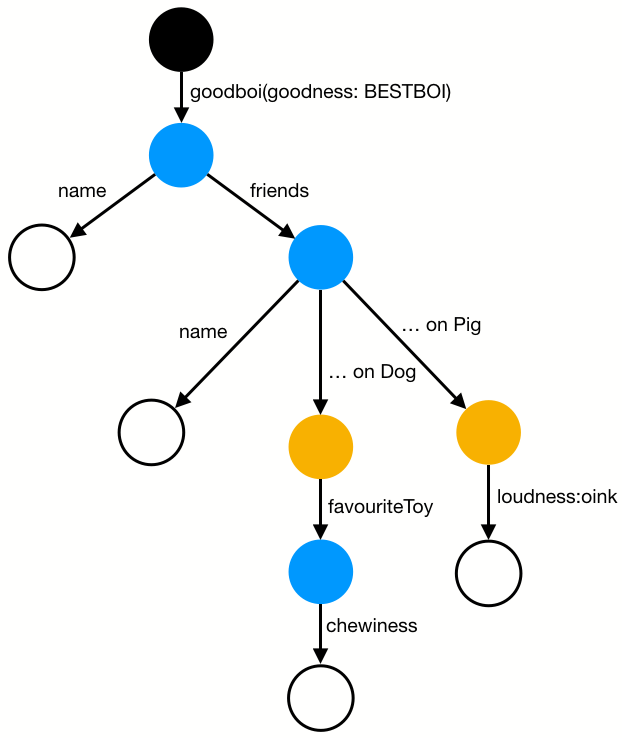
\includegraphics[scale=0.33]{imgs/query_tree.png}
    \caption{GraphQL query as a tree.}
    \label{fig:query_tree}
\end{figure}

Similar to the schema definition, we follow the \spec{}'s grammar as closely as possible, as can be seen from Figure~\ref{fig:query_def}. We do not embed the property of non-emptiness of subqueries in the definition because the \spec{} pushes it to a different validation rule, even though it is already embedded in the grammar, and we believe it is simpler to reuse the \texttt{seq} library and its existent functionalities. 

\begin{figure*}[h]
  \centering
  \begin{subfigure}{.5\textwidth}
    \begin{grammar}
        <Query> ::= <name> \textbf{\texttt{(}} <Arg>* \textbf{\texttt{)}}
        \alt <alias> \textbf{\texttt{:}} <name> \textbf{\texttt{(}} <Arg>* \textbf{\texttt{)}}
        \alt <name> \textbf{(} <Arg>* \textbf{)} \textbf{\texttt{\{}} <Query>$^{+}$ \textbf{\texttt{\}}}
        \alt <alias> \textbf{\texttt{:}} <name> \textbf{\texttt{(}} <Arg>* \textbf{\texttt{)}} \textbf{\texttt{\{}} <Query>$^{+}$ \textbf{\texttt{\}}}
        \alt \textbf{\texttt{... on}} <name> \textbf{\texttt{\{}} <Query>$^{+}$ \textbf{\texttt{\}}}
        
        <Arg> ::= <name> \textbf{\texttt{:}} <value>
    \end{grammar}
  \end{subfigure}%
  \begin{subfigure}{.5\textwidth}

    \begin{minted}{coq}
    Inductive Query : Type :=
    | SingleField (name : Name)
                  (arguments : seq (Name * Vals))
    | AliasedField (alias : Name)
                   (name : Name)
                   (arguments : seq (Name * Vals))
    | NestedField (name : Name)
                  (arguments : seq (Name * Vals))
                  (subqueries : seq Query)
    | NestedAliasedField (alias : Name)
                         (name : Name)
                         (arguments : seq (Name * Vals))
                         (subqueries : seq Query)
    | InlineFragment (type_condition : Name)
                     (subqueries : seq Query).
    \end{minted}
  \end{subfigure}
  \caption{Definition of GraphQL queries, the \spec{}'s grammar (left) and the Coq implementation (right).}
  \label{fig:query_def}
\end{figure*}


The definition of queries is completely independent of any schema, both in the \spec{} and our formalization, thus requiring a validation process to establish a proper relation. We define the property of \textit{conformance} of queries, based on validation rules scattered throughout the \textit{Validation} section of the \spec{}\footnote{https://graphql.github.io/graphql-spec/June2018/\#sec-Validation}. The validity of queries depends on the notion of the \textit{type in context} where queries are defined\footnote{The \spec{} refers to it as type in scope or parent type. Some algorithmic descriptions make use of the types in context but are not explicit in their signatures.}. Since queries are selections over the fields of types, it is important to know exactly to what type they are being applied. Consider the following query where there are two occurrences of the field \texttt{name}. In one case, the field is requesting information about the \texttt{Dog} type, while in the other it is used in the context of the \texttt{Pig} type. The distinction is important because some selections might be valid in some contexts but not in others, such as the case of the field \texttt{favoriteToy} that is valid in the context of a \texttt{Dog} type but should not be requested of a \texttt{Pig} type. Similarly, a field may be defined in two separate types and have different return types in each, as shown below in the field \texttt{age} of the types \texttt{Human} and \texttt{Martian}.

%Just as in the case of well-formedness of schemas or conformance of graphs, queries must go through a validation process. We define the property of \textit{conformance} of queries, based on validation rules scattered throughout the \textit{Validation} section of the \spec{}\footnote{https://graphql.github.io/graphql-spec/June2018/\#sec-Validation}.

% Before describing the validation process, it is very important to address the notion of \textit{type in context} where queries are defined and used. The type in context is the type over which a user might be requesting information on its fields. To illustrate this, consider the following query. The first selection, namely \texttt{goodboi}, is requesting information about the query type, meaning that it is used in the context of the \texttt{Query} type. Moving onto the  \texttt{name} subselection, it is not direct which is. In one case, the type in context is \texttt{Dog}, while in the other the field is used in the context of the \texttt{Pig} type.

\begin{minted}[escapeinside=||, mathescape=true]{js}
      query {
        goodboi {
          |$\ldots$| on Dog {
            name
            favoriteToy
          }
          |$\ldots$| on Pig {
            name
            favoriteToy
          }
        }
      }
      
      type Human {
        age: Int
      }

      type Martian {
        age: Float
      }	
\end{minted}

% The importance of this type in context is that fields or inline fragments might be valid in certain cases but not in others. Similarly, a field may have a particular return type in one case and a different one in another type, like in the following example. Both types have an \texttt{age} field, but in one case it returns an integer value while in the other a floating point value. If that field is encountered in a query, it is necessary to know to which type it is being requested.



\begin{definition}
A GraphQL query $\varphi$ \textit{conforms} to a schema $\mathcal{S}$ if it satisfies the following conditions:
\begin{itemize}
    \item Selections in $\varphi$ are consistent.

    \item Field merging between fields is possible.
    % During the evaluation process, fields with the same response name are collected and merged to ensure that they are all executed at the same time. This validation rule checks that it makes sense to merge those fields. The following example illustrates two queries that have the same response name but should not be merged. The first one is accessing the field \texttt{name} while the second is accessing the field \texttt{age} but renaming it to \texttt{name}. Both are selections on different fields of the same type but with the same response name.
    % \begin{minted}{graphql}
    %                query {
    %                    name
    %                    name:age
    %                }
    %\end{minted}

    \item Fields with same response name have compatible response shapes.
    % This checks whether two fields with the same response name will produce response values that are consistent to each other. These values should be unambiguous for a user. For instance, the following example\td{These examples look a bit off I think.} shows two queries that produce similar responses but with ambiguous values. In the first one, we ask for dog's \texttt{name}s, which are strings, and in the second for pig's \texttt{age}s, which are integers. We also rename the \texttt{age} value to \texttt{name}. The responses we get will have some cases where \texttt{name} is associated to a string and other where it is associated to integers.
    % \begin{minted}[escapeinside=||,mathescape=true]{graphql}
    %                query {
    %                    |$\ldots$| on Dog {
    %                        name
    %                    }
    %                    |$\ldots$| on Pig {
    %                        name:age
    %                    }
    %                }
    % \end{minted}
\end{itemize}
\end{definition}

The implementation can be seen in the code below, however due to space limitations we only informally describe the three mentioned rules. The complete definitions can be found in the file \texttt{QueryConformance.v}.

\begin{minted}{coq}
Definition queries_conform (type_in_scope : Name)
                           (queries : seq Query) : bool :=
        all (is_consistent type_in_scope) queries &&
        is_field_merging_possible type_in_scope queries &&
        have_compatible_response_shapes
            [seq (type_in_scope, q) | q <- queries].
\end{minted}



The first rule specifies when a selection holds by itself, by checking aspects such as if query is over a field, then that field must be defined in the  type in context and its arguments are defined in the given field. Likewise, if a selection is an inline fragment, then the type condition has to be valid with respect to the type in context. The \spec{} defines this rule in several different sections.

The second validates when fields can be correctly merged during evaluation, which is an essential aspect of the semantics, since it ensures that repeated fields are only evaluated once. To illustrate this, consider the following query, where a user requests information on the fields \texttt{name} and \texttt{oink} of pigs. The user decides to rename the field \texttt{oink} to \texttt{name}, however this is invalid, since both fields cannot be merged and evaluated once; both fields refer to distinct pieces of information in the system.

\begin{minted}[escapeinside=||,mathescape=true]{js}
query {
	goodboi {
		|$\ldots$| on Pig {
			name
			name:oink
		}
	}
}
\end{minted}

The last rule is necessary to check when fields generate unambiguous outputs when evaluated. For instance, in the query below a user might request the names of dogs and the oinkness of pigs, but renaming the latter to have the same response name as the former. This query is considered invalid because evaluating it might produce a response that contains entries where the key \texttt{name} is associated to both string values and floating point numbers. 

\begin{minted}[escapeinside=||,mathescape=true]{js}
query {
	goodboi {
		friends {
			|$\ldots$| on Dog {
				name
			}
			|$\ldots$| on Pig {
				name:oink
			}
		}
	}
}

// Possible output

{
	"goodboi" : {
		"friends" : [
				{
					"name" : "Marle"
				},
				{
					"name" : 9000
				}
		]
	}
}
\end{minted}



				
These last two rules, for merging and unambiguous values, are defined as a single validation rule in the \spec{}\footnote{https://graphql.github.io/graphql-spec/June2018/\#sec-Field-Selection-Merging}, however we decide to separate them. The first reason, which we cover more extensively in Section~\ref{sec:discussion}, is that it is possible to optimize the algorithm by reducing redundant recursive calls. Secondly, splitting facilitates reasoning about the predicates.

% The main issue is that the \spec{} allows for what we call \textit{invalid fragments}, originally described in an issue in the \spec{}'s repository\footnote{https://github.com/graphql/graphql-spec/issues/367}. In a nutshell, the \spec{} allows using fragments with type conditions that can span to multiple unrelated types. These end up not being evaluated due to posterior checks\footnote{https://graphql.github.io/graphql-spec/June2018/\#DoesFragmentTypeApply()}.


This concludes the definition of GraphQL queries and the validation process. \td{Examples can be found in the files \texttt{SpecExamples.v} and \texttt{HPExample.v}}. For the rest of the paper, it is assumed that queries conform to a given schema. 

\subsection{Semantics}\label{subsec:semantics}

In this section we describe the semantics of GraphQL queries. We begin by briefly examining the responses generated by executing queries and then we give an informal description of the semantics, finishing with the formal definition. %We finish by discussing some implementation choices and comparison with the \spec{} and \HP{}.

We model responses to GraphQL queries with a tree structure, similar to JSON. We choose this structure to preserve similarity to queries and because it provides a strong reasoning principle, as well as being simpler to preserve order of the responses. This differs slightly from the \spec{}, which only states that responses are a map and does not impose an ordering of responses, although encourages it\footnote{https://graphql.github.io/graphql-spec/June2018/\#sec-Serialized-Map-Ordering}. We believe that preserving the order is one of the strong selling points for GraphQL (queries and their responses are very similar and easy to read). 

\td{Move to discussion?} Our approach has two main disadvantages: possible duplication of response names and cost of access. Since we use lists instead of maps, we can encounter duplicated names and accessing a value has a linear cost given by the lists size, instead of the constant access obtainable with a map. We still argue that the reasoning principles and simplicity to order is highly valuable. Nevertheless, we include a proof that the results obtained with the semantics have no duplicated names. Finally, we use option types to represent null values in the leaves of the response tree.

\begin{minted}{coq}
Inductive ResponseNode (A : Type) : Type :=
| Leaf : A -> ResponseNode
| Object : seq (Name * ResponseNode) -> ResponseNode
| Array : seq ResponseNode -> ResponseNode.

Definition GraphQLResponse (Vals: eqType) :=
    seq (Name * (@ResponseNode (option Vals))).
\end{minted}


As we described in Section~\ref{subsec:graph}, the underlying data model we use is a graph, therefore the semantics are instantiated to this setting. %In a following paragraph we briefly explore an alternative that is closer to the \spec{}, in the sense that it can be detached from a particular data model. 
Informally, the evaluation of a query then represents a navigation over a graph. At top level, a query begins from the root node and then navigates around its edges and nodes, collecting data along the way. In this sense:
\begin{itemize}
    \item A field selection represents either accessing a node's property or traversing an edge to a neighboring node.
    \item An inline fragment conditions whether using a node to access its properties or to traverse to other nodes.
    \item Subqueries are evaluated in neighboring nodes.
\end{itemize}

The formal definition of the semantics is depicted in Figure \ref{fig:semantics}. The definition displays the cases where a field selection is accessing a node's property, when it is navigating to other nodes and when it is evaluating an inline fragment. Aliased fields are omitted for brevity but the complete definition can be explored in the file \texttt{QuerySemantics.v}.

\td{Move to discussion?}
The main difference with respect to \HP{} and the main similarity to the \spec{} is that we perform a collection of fields at the query level, whereas \HP{} performs a post-processing of responses. The main reasons are our approach is more similar to the \spec{} and that it is harder to reason using \HP{}'s approach.

\td{Don't know how to present this or if it is relevant but I include it so you know it exists - The spec first groups fields by name and then evaluates each group. These are different steps. We define everything in one place because it was easier to reason about the semantics. The difficulty with the spec's approach is that when proving things about the semantics, you have to provide, at each step, the information on how your data is structured (every group contains only fields and every field in a group has the same response name as the group's key used to group them). This is problematic mostly because of inline fragments, which do not have response names. Definitions must always account for the case of inline fragments, even when they are thought out to be used only on fields. Our definition is maybe less compositional but thanks to Equations, it is simpler to reason about it - because Equations generate a nice reasoning principle. We also attempted defining it similarly to the spec, still preserving the information on the structure by using dependent types and Equation, but the resulting reasoning principle would end up being huge (80-100 cases) (I believe I read Matthieu saying that nesting some definitions could exponentially increase the size of the reasoning principle, which is what would occur in this case).}

%Our first attempt at defining the semantics was to follow \HP{}'s post-processing approach. Our intention was to be as close as possible to their formalization to later prove their transformation and equivalence results, which we cover in Section~\ref{sec:norm}. However, the non-structural recursive nature of both the transformations and the post-processing function made reasoning about semantic equivalence very hard.

\begin{figure*}[h]
    \centering
    \begin{align}
    % Empty
    \eval{\cdot}{u} &= [\cdot] \\
    % SingleField
    \evalu{\fld\; ::\; \queries} &= \begin{cases}
    \resp{\texttt{coerce(\val)}} \; ::\; \evalfilteru{\queries}{\fkey}  & \mathit{u.property}(\fld) = \val \\
    \resp{\nval} \; :: \; \evalfilteru{\queries}{\fkey} & \sim
    \end{cases}\\
    % Nested field
    \evalu{\nfld{\overline{\beta}} \; ::\; \queries} &=
    \begin{cases}
    \resp{\texttt{[} \mathit{map} (\lambda\; v_{i} \Rightarrow \eval{\overline{\beta} \mdoubleplus \mathit{merge (collect_\fkey (\queries))}}{v_{i}})\; \mathit{neighbors(u)} \texttt{]}} \; :: \; \evalfilteru{\queries}{f}  & \mathit{type(f)} \in L_{t} \text{and} \{v_{1}, \ldots, v_{k}\} = \{v_{i} \mid (u, f[\alpha], v_{i}) \in E\} \\
    (f:\{\eval{\subqueries{\beta}}{v}\})\; :: \; \evalfilteru{\queries}{f}  & \mathit{type(f)} \notin L_{t} \text{and} (u, f[\alpha], v) \in E \\
    (f:null)\; :: \; \evalfilteru{\queries}{f} & \mathit{type(f)} \notin L_{t} \text{and there is no } v \text{ s.t.} (u, f[\alpha], v) \in E \\
    \end{cases}\\
    %inline fragment
    \evalu{\ifrag{t}{\overline{\beta}}\; ::\; \queries} &= \begin{cases}
    \evalu{\overline{\beta} \mdoubleplus \queries} & \mathit{does\_fragment\_type\_apply_{\texttt{t}}(u.type)} = \texttt{true}\\
    \evalu{\queries} & \sim
    \end{cases}
    \end{align}
    \caption{Semantics for GraphQL queries.\td{This looks bad but I don't know how to format it :/}}
    \label{fig:semantics}
\end{figure*}

%The first one is that we currently do not handle errors during execution. This is due to two main reasons: the evaluation function assumes it receives valid queries and we have not yet implemented non-null types. These relates to the two kinds of errors one may encounter when evaluating GraphQL queries: validation and execution errors. The first ones are captured before execution and displayed to the user. Our semantics has to deal with a case which would be ruled out by the validation process. We believe both cases can be covered by including X (monad/reasonably exceptional type theory/etc)\td{rewrite}.

% The second major aspect refers to completeness. Both our formalization and \HP{}'s do not generate all possible results expected by a GraphQL service. In particular, there is a limitation when generating lists with a nesting bigger than one. it does not generate results for list types of depth bigger than one, when its inner type is not a scalar type\footnote{HP goes a step further and does not allow any type of nested list result.}. For instance, one might want to get information about friends but grouped by their age. This could be modeled as a field with type \texttt{[[Human]]}, where the list type has depth 2. A response for this query would look something like \texttt{"friends":[[...], ..., [...]]}. This response cannot be generated by our semantics\footnote{It can be defined with the \mintinline{coq}{Response} structure but not generated with the semantics.}.

%The main challenge in this case is to define what this nested list types represent in a graph. If we take a simple case of a field with type \texttt{[Human]}, we can model it as neighbors of a node. However, if we increase the nesting such as \texttt{[[Human]]}, it becomes harder to model. What does this represent in the graph? Should we introduce blank nodes in between the source node and the \texttt{Human} nodes? Are these inner edges labeled? Should there be a blank node per each level of nesting or a single one with edges to itself? All these questions do not have a straightforward answer. Our semantics, as the one definded in PH, simply ignores any nesting bigger than one.\td{This is where it can be modelled using Functors. The \spec{} checks if it received a collection and applies map to eventually get to the concrete values. Not sure how to put this out there.}

This concludes the base formalization of GraphQL schemas, graph data model, and queries and their semantics.  These definitions provide the base upon which further development and analysis can be developed.

\td{I feel there is not much to say about the semantics... The "juicy" bits are in the discussion section - limitations given by the graph model, functor approach to the spec's semantics, etc.}
